\documentclass[]{article}
\usepackage{lmodern}
\usepackage{amssymb,amsmath}
\usepackage{ifxetex,ifluatex}
\usepackage{fixltx2e} % provides \textsubscript
\ifnum 0\ifxetex 1\fi\ifluatex 1\fi=0 % if pdftex
  \usepackage[T1]{fontenc}
  \usepackage[utf8]{inputenc}
\else % if luatex or xelatex
  \ifxetex
    \usepackage{mathspec}
  \else
    \usepackage{fontspec}
  \fi
  \defaultfontfeatures{Ligatures=TeX,Scale=MatchLowercase}
\fi
% use upquote if available, for straight quotes in verbatim environments
\IfFileExists{upquote.sty}{\usepackage{upquote}}{}
% use microtype if available
\IfFileExists{microtype.sty}{%
\usepackage{microtype}
\UseMicrotypeSet[protrusion]{basicmath} % disable protrusion for tt fonts
}{}
\usepackage[margin=1in]{geometry}
\usepackage{hyperref}
\hypersetup{unicode=true,
            pdftitle={Multiple linear regression},
            pdfauthor={Jimmy Ng},
            pdfborder={0 0 0},
            breaklinks=true}
\urlstyle{same}  % don't use monospace font for urls
\usepackage{color}
\usepackage{fancyvrb}
\newcommand{\VerbBar}{|}
\newcommand{\VERB}{\Verb[commandchars=\\\{\}]}
\DefineVerbatimEnvironment{Highlighting}{Verbatim}{commandchars=\\\{\}}
% Add ',fontsize=\small' for more characters per line
\usepackage{framed}
\definecolor{shadecolor}{RGB}{248,248,248}
\newenvironment{Shaded}{\begin{snugshade}}{\end{snugshade}}
\newcommand{\KeywordTok}[1]{\textcolor[rgb]{0.13,0.29,0.53}{\textbf{#1}}}
\newcommand{\DataTypeTok}[1]{\textcolor[rgb]{0.13,0.29,0.53}{#1}}
\newcommand{\DecValTok}[1]{\textcolor[rgb]{0.00,0.00,0.81}{#1}}
\newcommand{\BaseNTok}[1]{\textcolor[rgb]{0.00,0.00,0.81}{#1}}
\newcommand{\FloatTok}[1]{\textcolor[rgb]{0.00,0.00,0.81}{#1}}
\newcommand{\ConstantTok}[1]{\textcolor[rgb]{0.00,0.00,0.00}{#1}}
\newcommand{\CharTok}[1]{\textcolor[rgb]{0.31,0.60,0.02}{#1}}
\newcommand{\SpecialCharTok}[1]{\textcolor[rgb]{0.00,0.00,0.00}{#1}}
\newcommand{\StringTok}[1]{\textcolor[rgb]{0.31,0.60,0.02}{#1}}
\newcommand{\VerbatimStringTok}[1]{\textcolor[rgb]{0.31,0.60,0.02}{#1}}
\newcommand{\SpecialStringTok}[1]{\textcolor[rgb]{0.31,0.60,0.02}{#1}}
\newcommand{\ImportTok}[1]{#1}
\newcommand{\CommentTok}[1]{\textcolor[rgb]{0.56,0.35,0.01}{\textit{#1}}}
\newcommand{\DocumentationTok}[1]{\textcolor[rgb]{0.56,0.35,0.01}{\textbf{\textit{#1}}}}
\newcommand{\AnnotationTok}[1]{\textcolor[rgb]{0.56,0.35,0.01}{\textbf{\textit{#1}}}}
\newcommand{\CommentVarTok}[1]{\textcolor[rgb]{0.56,0.35,0.01}{\textbf{\textit{#1}}}}
\newcommand{\OtherTok}[1]{\textcolor[rgb]{0.56,0.35,0.01}{#1}}
\newcommand{\FunctionTok}[1]{\textcolor[rgb]{0.00,0.00,0.00}{#1}}
\newcommand{\VariableTok}[1]{\textcolor[rgb]{0.00,0.00,0.00}{#1}}
\newcommand{\ControlFlowTok}[1]{\textcolor[rgb]{0.13,0.29,0.53}{\textbf{#1}}}
\newcommand{\OperatorTok}[1]{\textcolor[rgb]{0.81,0.36,0.00}{\textbf{#1}}}
\newcommand{\BuiltInTok}[1]{#1}
\newcommand{\ExtensionTok}[1]{#1}
\newcommand{\PreprocessorTok}[1]{\textcolor[rgb]{0.56,0.35,0.01}{\textit{#1}}}
\newcommand{\AttributeTok}[1]{\textcolor[rgb]{0.77,0.63,0.00}{#1}}
\newcommand{\RegionMarkerTok}[1]{#1}
\newcommand{\InformationTok}[1]{\textcolor[rgb]{0.56,0.35,0.01}{\textbf{\textit{#1}}}}
\newcommand{\WarningTok}[1]{\textcolor[rgb]{0.56,0.35,0.01}{\textbf{\textit{#1}}}}
\newcommand{\AlertTok}[1]{\textcolor[rgb]{0.94,0.16,0.16}{#1}}
\newcommand{\ErrorTok}[1]{\textcolor[rgb]{0.64,0.00,0.00}{\textbf{#1}}}
\newcommand{\NormalTok}[1]{#1}
\usepackage{longtable,booktabs}
\usepackage{graphicx,grffile}
\makeatletter
\def\maxwidth{\ifdim\Gin@nat@width>\linewidth\linewidth\else\Gin@nat@width\fi}
\def\maxheight{\ifdim\Gin@nat@height>\textheight\textheight\else\Gin@nat@height\fi}
\makeatother
% Scale images if necessary, so that they will not overflow the page
% margins by default, and it is still possible to overwrite the defaults
% using explicit options in \includegraphics[width, height, ...]{}
\setkeys{Gin}{width=\maxwidth,height=\maxheight,keepaspectratio}
\IfFileExists{parskip.sty}{%
\usepackage{parskip}
}{% else
\setlength{\parindent}{0pt}
\setlength{\parskip}{6pt plus 2pt minus 1pt}
}
\setlength{\emergencystretch}{3em}  % prevent overfull lines
\providecommand{\tightlist}{%
  \setlength{\itemsep}{0pt}\setlength{\parskip}{0pt}}
\setcounter{secnumdepth}{0}
% Redefines (sub)paragraphs to behave more like sections
\ifx\paragraph\undefined\else
\let\oldparagraph\paragraph
\renewcommand{\paragraph}[1]{\oldparagraph{#1}\mbox{}}
\fi
\ifx\subparagraph\undefined\else
\let\oldsubparagraph\subparagraph
\renewcommand{\subparagraph}[1]{\oldsubparagraph{#1}\mbox{}}
\fi

%%% Use protect on footnotes to avoid problems with footnotes in titles
\let\rmarkdownfootnote\footnote%
\def\footnote{\protect\rmarkdownfootnote}

%%% Change title format to be more compact
\usepackage{titling}

% Create subtitle command for use in maketitle
\newcommand{\subtitle}[1]{
  \posttitle{
    \begin{center}\large#1\end{center}
    }
}

\setlength{\droptitle}{-2em}

  \title{Multiple linear regression}
    \pretitle{\vspace{\droptitle}\centering\huge}
  \posttitle{\par}
    \author{Jimmy Ng}
    \preauthor{\centering\large\emph}
  \postauthor{\par}
      \predate{\centering\large\emph}
  \postdate{\par}
    \date{November 2, 2018}


\begin{document}
\maketitle

\subsection{Grading the professor}\label{grading-the-professor}

Many college courses conclude by giving students the opportunity to
evaluate the course and the instructor anonymously. However, the use of
these student evaluations as an indicator of course quality and teaching
effectiveness is often criticized because these measures may reflect the
influence of non-teaching related characteristics, such as the physical
appearance of the instructor. The article titled, ``Beauty in the
classroom: instructors' pulchritude and putative pedagogical
productivity'' (Hamermesh and Parker, 2005) found that instructors who
are viewed to be better looking receive higher instructional ratings.
(Daniel S. Hamermesh, Amy Parker, Beauty in the classroom: instructors
pulchritude and putative pedagogical productivity, \emph{Economics of
Education Review}, Volume 24, Issue 4, August 2005, Pages 369-376, ISSN
0272-7757, 10.1016/j.econedurev.2004.07.013.
\url{http://www.sciencedirect.com/science/article/pii/S0272775704001165}.)

In this lab we will analyze the data from this study in order to learn
what goes into a positive professor evaluation.

\subsection{The data}\label{the-data}

The data were gathered from end of semester student evaluations for a
large sample of professors from the University of Texas at Austin. In
addition, six students rated the professors' physical appearance. (This
is aslightly modified version of the original data set that was released
as part of the replication data for \emph{Data Analysis Using Regression
and Multilevel/Hierarchical Models} (Gelman and Hill, 2007).) The result
is a data frame where each row contains a different course and columns
represent variables about the courses and professors.

\begin{Shaded}
\begin{Highlighting}[]
\KeywordTok{load}\NormalTok{(}\StringTok{"more/evals.RData"}\NormalTok{)}
\end{Highlighting}
\end{Shaded}

\begin{longtable}[]{@{}ll@{}}
\toprule
\begin{minipage}[b]{0.22\columnwidth}\raggedright\strut
variable\strut
\end{minipage} & \begin{minipage}[b]{0.16\columnwidth}\raggedright\strut
description\strut
\end{minipage}\tabularnewline
\midrule
\endhead
\begin{minipage}[t]{0.22\columnwidth}\raggedright\strut
\texttt{score}\strut
\end{minipage} & \begin{minipage}[t]{0.16\columnwidth}\raggedright\strut
average professor evaluation score: (1) very unsatisfactory - (5)
excellent.\strut
\end{minipage}\tabularnewline
\begin{minipage}[t]{0.22\columnwidth}\raggedright\strut
\texttt{rank}\strut
\end{minipage} & \begin{minipage}[t]{0.16\columnwidth}\raggedright\strut
rank of professor: teaching, tenure track, tenured.\strut
\end{minipage}\tabularnewline
\begin{minipage}[t]{0.22\columnwidth}\raggedright\strut
\texttt{ethnicity}\strut
\end{minipage} & \begin{minipage}[t]{0.16\columnwidth}\raggedright\strut
ethnicity of professor: not minority, minority.\strut
\end{minipage}\tabularnewline
\begin{minipage}[t]{0.22\columnwidth}\raggedright\strut
\texttt{gender}\strut
\end{minipage} & \begin{minipage}[t]{0.16\columnwidth}\raggedright\strut
gender of professor: female, male.\strut
\end{minipage}\tabularnewline
\begin{minipage}[t]{0.22\columnwidth}\raggedright\strut
\texttt{language}\strut
\end{minipage} & \begin{minipage}[t]{0.16\columnwidth}\raggedright\strut
language of school where professor received education: english or
non-english.\strut
\end{minipage}\tabularnewline
\begin{minipage}[t]{0.22\columnwidth}\raggedright\strut
\texttt{age}\strut
\end{minipage} & \begin{minipage}[t]{0.16\columnwidth}\raggedright\strut
age of professor.\strut
\end{minipage}\tabularnewline
\begin{minipage}[t]{0.22\columnwidth}\raggedright\strut
\texttt{cls\_perc\_eval}\strut
\end{minipage} & \begin{minipage}[t]{0.16\columnwidth}\raggedright\strut
percent of students in class who completed evaluation.\strut
\end{minipage}\tabularnewline
\begin{minipage}[t]{0.22\columnwidth}\raggedright\strut
\texttt{cls\_did\_eval}\strut
\end{minipage} & \begin{minipage}[t]{0.16\columnwidth}\raggedright\strut
number of students in class who completed evaluation.\strut
\end{minipage}\tabularnewline
\begin{minipage}[t]{0.22\columnwidth}\raggedright\strut
\texttt{cls\_students}\strut
\end{minipage} & \begin{minipage}[t]{0.16\columnwidth}\raggedright\strut
total number of students in class.\strut
\end{minipage}\tabularnewline
\begin{minipage}[t]{0.22\columnwidth}\raggedright\strut
\texttt{cls\_level}\strut
\end{minipage} & \begin{minipage}[t]{0.16\columnwidth}\raggedright\strut
class level: lower, upper.\strut
\end{minipage}\tabularnewline
\begin{minipage}[t]{0.22\columnwidth}\raggedright\strut
\texttt{cls\_profs}\strut
\end{minipage} & \begin{minipage}[t]{0.16\columnwidth}\raggedright\strut
number of professors teaching sections in course in sample: single,
multiple.\strut
\end{minipage}\tabularnewline
\begin{minipage}[t]{0.22\columnwidth}\raggedright\strut
\texttt{cls\_credits}\strut
\end{minipage} & \begin{minipage}[t]{0.16\columnwidth}\raggedright\strut
number of credits of class: one credit (lab, PE, etc.), multi
credit.\strut
\end{minipage}\tabularnewline
\begin{minipage}[t]{0.22\columnwidth}\raggedright\strut
\texttt{bty\_f1lower}\strut
\end{minipage} & \begin{minipage}[t]{0.16\columnwidth}\raggedright\strut
beauty rating of professor from lower level female: (1) lowest - (10)
highest.\strut
\end{minipage}\tabularnewline
\begin{minipage}[t]{0.22\columnwidth}\raggedright\strut
\texttt{bty\_f1upper}\strut
\end{minipage} & \begin{minipage}[t]{0.16\columnwidth}\raggedright\strut
beauty rating of professor from upper level female: (1) lowest - (10)
highest.\strut
\end{minipage}\tabularnewline
\begin{minipage}[t]{0.22\columnwidth}\raggedright\strut
\texttt{bty\_f2upper}\strut
\end{minipage} & \begin{minipage}[t]{0.16\columnwidth}\raggedright\strut
beauty rating of professor from second upper level female: (1) lowest -
(10) highest.\strut
\end{minipage}\tabularnewline
\begin{minipage}[t]{0.22\columnwidth}\raggedright\strut
\texttt{bty\_m1lower}\strut
\end{minipage} & \begin{minipage}[t]{0.16\columnwidth}\raggedright\strut
beauty rating of professor from lower level male: (1) lowest - (10)
highest.\strut
\end{minipage}\tabularnewline
\begin{minipage}[t]{0.22\columnwidth}\raggedright\strut
\texttt{bty\_m1upper}\strut
\end{minipage} & \begin{minipage}[t]{0.16\columnwidth}\raggedright\strut
beauty rating of professor from upper level male: (1) lowest - (10)
highest.\strut
\end{minipage}\tabularnewline
\begin{minipage}[t]{0.22\columnwidth}\raggedright\strut
\texttt{bty\_m2upper}\strut
\end{minipage} & \begin{minipage}[t]{0.16\columnwidth}\raggedright\strut
beauty rating of professor from second upper level male: (1) lowest -
(10) highest.\strut
\end{minipage}\tabularnewline
\begin{minipage}[t]{0.22\columnwidth}\raggedright\strut
\texttt{bty\_avg}\strut
\end{minipage} & \begin{minipage}[t]{0.16\columnwidth}\raggedright\strut
average beauty rating of professor.\strut
\end{minipage}\tabularnewline
\begin{minipage}[t]{0.22\columnwidth}\raggedright\strut
\texttt{pic\_outfit}\strut
\end{minipage} & \begin{minipage}[t]{0.16\columnwidth}\raggedright\strut
outfit of professor in picture: not formal, formal.\strut
\end{minipage}\tabularnewline
\begin{minipage}[t]{0.22\columnwidth}\raggedright\strut
\texttt{pic\_color}\strut
\end{minipage} & \begin{minipage}[t]{0.16\columnwidth}\raggedright\strut
color of professor's picture: color, black \& white.\strut
\end{minipage}\tabularnewline
\bottomrule
\end{longtable}

\subsection{Exploring the data}\label{exploring-the-data}

\begin{enumerate}
\def\labelenumi{\arabic{enumi}.}
\item
  Is this an observational study or an experiment? The original research
  question posed in the paper is whether beauty leads directly to the
  differences in course evaluations. Given the study design, is it
  possible to answer this question as it is phrased? If not, rephrase
  the question. \# JN: strictly speaking, this is an observational study
  because we do not control about assigning students to different
  professors/classes. What if all English professors are considered to
  be significantly more attractive than professors teaching mathematics?
  Neither do we control the ``attractiveness'' of professors in this
  student. We cannot do randomized control trial. However, we can still
  answer the question by carrying out a correlation or
  quasi-experimental study.
\item
  Describe the distribution of \texttt{score}. Is the distribution
  skewed? What does that tell you about how students rate courses? Is
  this what you expected to see? Why, or why not?
\end{enumerate}

\begin{Shaded}
\begin{Highlighting}[]
\KeywordTok{par}\NormalTok{(}\DataTypeTok{mfrow =} \KeywordTok{c}\NormalTok{(}\DecValTok{1}\NormalTok{, }\DecValTok{2}\NormalTok{))}
\KeywordTok{hist}\NormalTok{(evals}\OperatorTok{$}\NormalTok{score, }\DataTypeTok{main =} \StringTok{"histogram of score"}\NormalTok{)}
\KeywordTok{boxplot}\NormalTok{(evals}\OperatorTok{$}\NormalTok{score, }\DataTypeTok{main =} \StringTok{"boxplot of score"}\NormalTok{)}
\end{Highlighting}
\end{Shaded}

\includegraphics{traveler-multiple_regression_files/figure-latex/unnamed-chunk-1-1.pdf}
\# JN: Yes that's heavily left skewed. That means majority of students
have positive rating of their professors, with only few exceptions that
rate their professors negatively (or below average). That's what I
expected - majority of students have positive learning experience.

\begin{enumerate}
\def\labelenumi{\arabic{enumi}.}
\setcounter{enumi}{2}
\tightlist
\item
  Excluding \texttt{score}, select two other variables and describe
  their relationship using an appropriate visualization (scatterplot,
  side-by-side boxplots, or mosaic plot).
\end{enumerate}

\begin{Shaded}
\begin{Highlighting}[]
\KeywordTok{with}\NormalTok{(evals, }
     \KeywordTok{plot}\NormalTok{(bty_avg }\OperatorTok{~}\StringTok{ }\NormalTok{age))}
\end{Highlighting}
\end{Shaded}

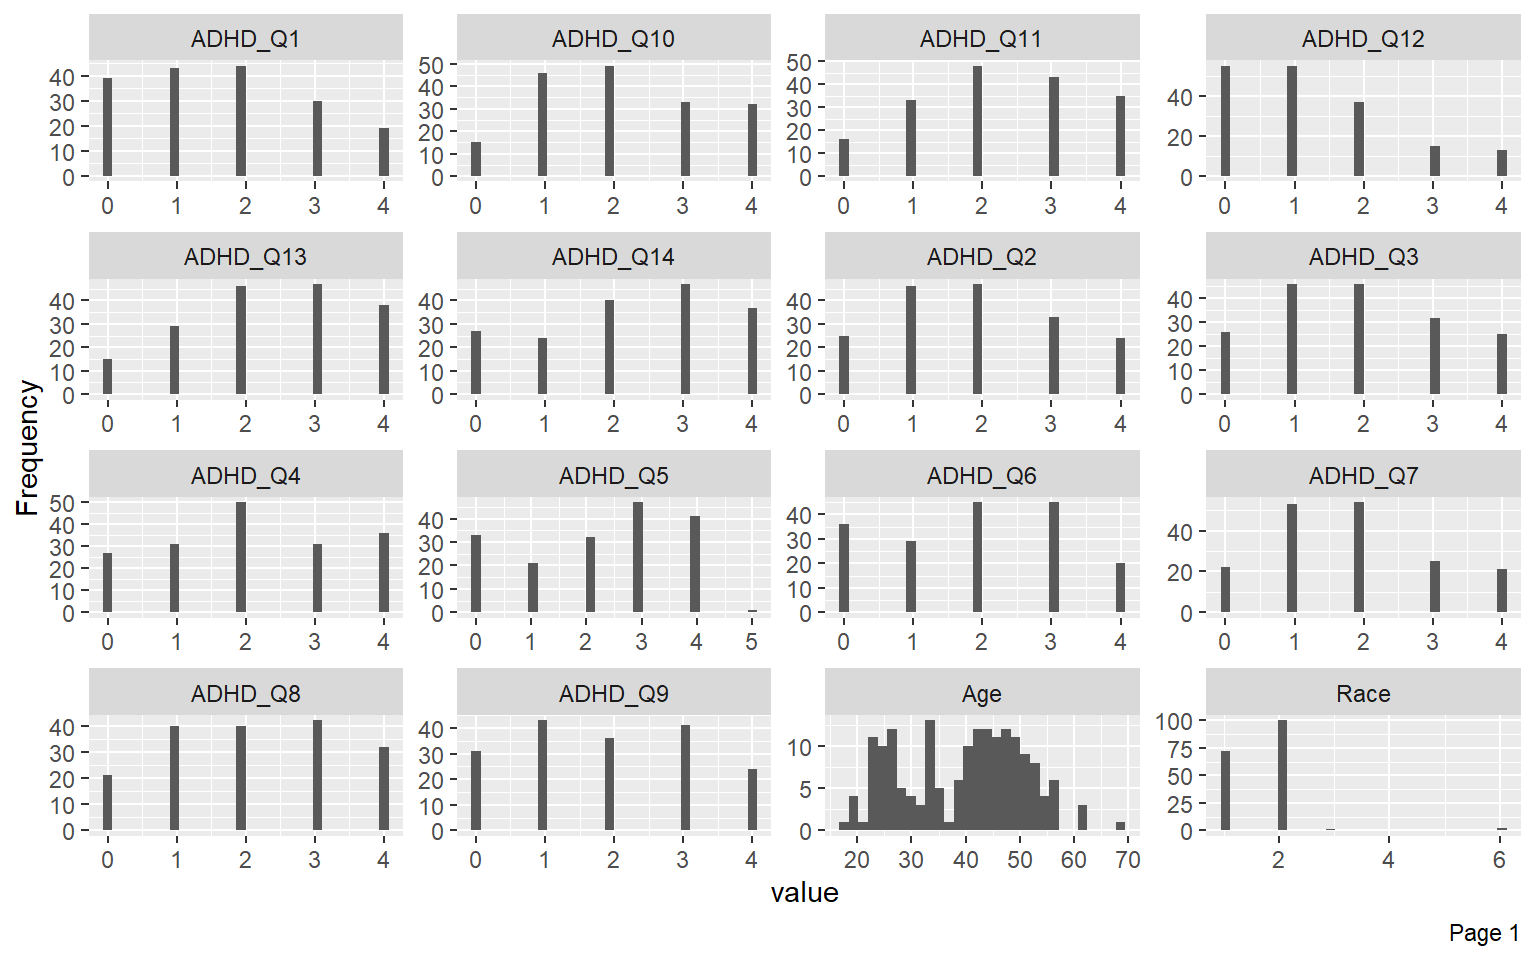
\includegraphics{traveler-multiple_regression_files/figure-latex/unnamed-chunk-2-1.pdf}

\begin{Shaded}
\begin{Highlighting}[]
\KeywordTok{with}\NormalTok{(evals,}
     \KeywordTok{cor.test}\NormalTok{(bty_avg, age))}
\NormalTok{## }
\NormalTok{##  Pearson's product-moment correlation}
\NormalTok{## }
\NormalTok{## data:  bty_avg and age}
\NormalTok{## t = -6.8664, df = 461, p-value = 2.137e-11}
\NormalTok{## alternative hypothesis: true correlation is not equal to 0}
\NormalTok{## 95 percent confidence interval:}
\NormalTok{##  -0.3850454 -0.2195681}
\NormalTok{## sample estimates:}
\NormalTok{##        cor }
\NormalTok{## -0.3046034}
\end{Highlighting}
\end{Shaded}

\section{JN: there's a very weak negative correlation between a
professor's age and his/her average beauty
rating.}\label{jn-theres-a-very-weak-negative-correlation-between-a-professors-age-and-hisher-average-beauty-rating.}

\subsection{Simple linear regression}\label{simple-linear-regression}

The fundamental phenomenon suggested by the study is that better looking
teachers are evaluated more favorably. Let's create a scatterplot to see
if this appears to be the case:

\begin{Shaded}
\begin{Highlighting}[]
\KeywordTok{plot}\NormalTok{(evals}\OperatorTok{$}\NormalTok{score }\OperatorTok{~}\StringTok{ }\NormalTok{evals}\OperatorTok{$}\NormalTok{bty_avg)}
\end{Highlighting}
\end{Shaded}

Before we draw conclusions about the trend, compare the number of
observations in the data frame with the approximate number of points on
the scatterplot. Is anything awry?

\begin{enumerate}
\def\labelenumi{\arabic{enumi}.}
\setcounter{enumi}{3}
\tightlist
\item
  Replot the scatterplot, but this time use the function
  \texttt{jitter()} on the \(y\)- or the \(x\)-coordinate. (Use
  \texttt{?jitter} to learn more.) What was misleading about the initial
  scatterplot?
\end{enumerate}

\begin{Shaded}
\begin{Highlighting}[]
\KeywordTok{plot}\NormalTok{(evals}\OperatorTok{$}\NormalTok{score }\OperatorTok{~}\StringTok{ }\KeywordTok{jitter}\NormalTok{(evals}\OperatorTok{$}\NormalTok{bty_avg))}
\end{Highlighting}
\end{Shaded}

\section{\texorpdfstring{JN: what's misleading about the scatterplot is
that, although the two variables look like ``continuous'', they are
actually not. If we run library(tidyverse), and then
``unique(evals\(bty_avg) %>% length" and "unique(evals\)bty\_avg)
\%\textgreater{}\% length'', we will see that we only have 27 uniques
for score and 35 for bty\_avg. In other words, there are ``spaces'' or
``gaps'' between dots and as a result, the scatterplot depicts the
relationship between the two variables visually less
convincing.}{JN: what's misleading about the scatterplot is that, although the two variables look like continuous, they are actually not. If we run library(tidyverse), and then unique(evalsbty\_avg) \%\textgreater{}\% length" and "unique(evalsbty\_avg) \%\textgreater{}\% length, we will see that we only have 27 uniques for score and 35 for bty\_avg. In other words, there are spaces or gaps between dots and as a result, the scatterplot depicts the relationship between the two variables visually less convincing.}}\label{jn-whats-misleading-about-the-scatterplot-is-that-although-the-two-variables-look-like-continuous-they-are-actually-not.-if-we-run-librarytidyverse-and-then-uniqueevalsbty_avg-length-and-uniqueevalsbty_avg-length-we-will-see-that-we-only-have-27-uniques-for-score-and-35-for-bty_avg.-in-other-words-there-are-spaces-or-gaps-between-dots-and-as-a-result-the-scatterplot-depicts-the-relationship-between-the-two-variables-visually-less-convincing.}

\begin{enumerate}
\def\labelenumi{\arabic{enumi}.}
\setcounter{enumi}{4}
\tightlist
\item
  Let's see if the apparent trend in the plot is something more than
  natural variation. Fit a linear model called \texttt{m\_bty} to
  predict average professor score by average beauty rating and add the
  line to your plot using \texttt{abline(m\_bty)}. Write out the
  equation for the linear model and interpret the slope. Is average
  beauty score a statistically significant predictor? Does it appear to
  be a practically significant predictor?
\end{enumerate}

\begin{Shaded}
\begin{Highlighting}[]
\NormalTok{m_bty <-}\StringTok{ }\KeywordTok{lm}\NormalTok{(score }\OperatorTok{~}\StringTok{ }\NormalTok{bty_avg, }\DataTypeTok{data =}\NormalTok{ evals)}
\KeywordTok{plot}\NormalTok{(}\KeywordTok{jitter}\NormalTok{(evals}\OperatorTok{$}\NormalTok{score) }\OperatorTok{~}\StringTok{ }\KeywordTok{jitter}\NormalTok{(evals}\OperatorTok{$}\NormalTok{bty_avg))}
\KeywordTok{abline}\NormalTok{(m_bty, }\DataTypeTok{lty =} \DecValTok{2}\NormalTok{, }\DataTypeTok{col =} \StringTok{"red"}\NormalTok{)}
\end{Highlighting}
\end{Shaded}

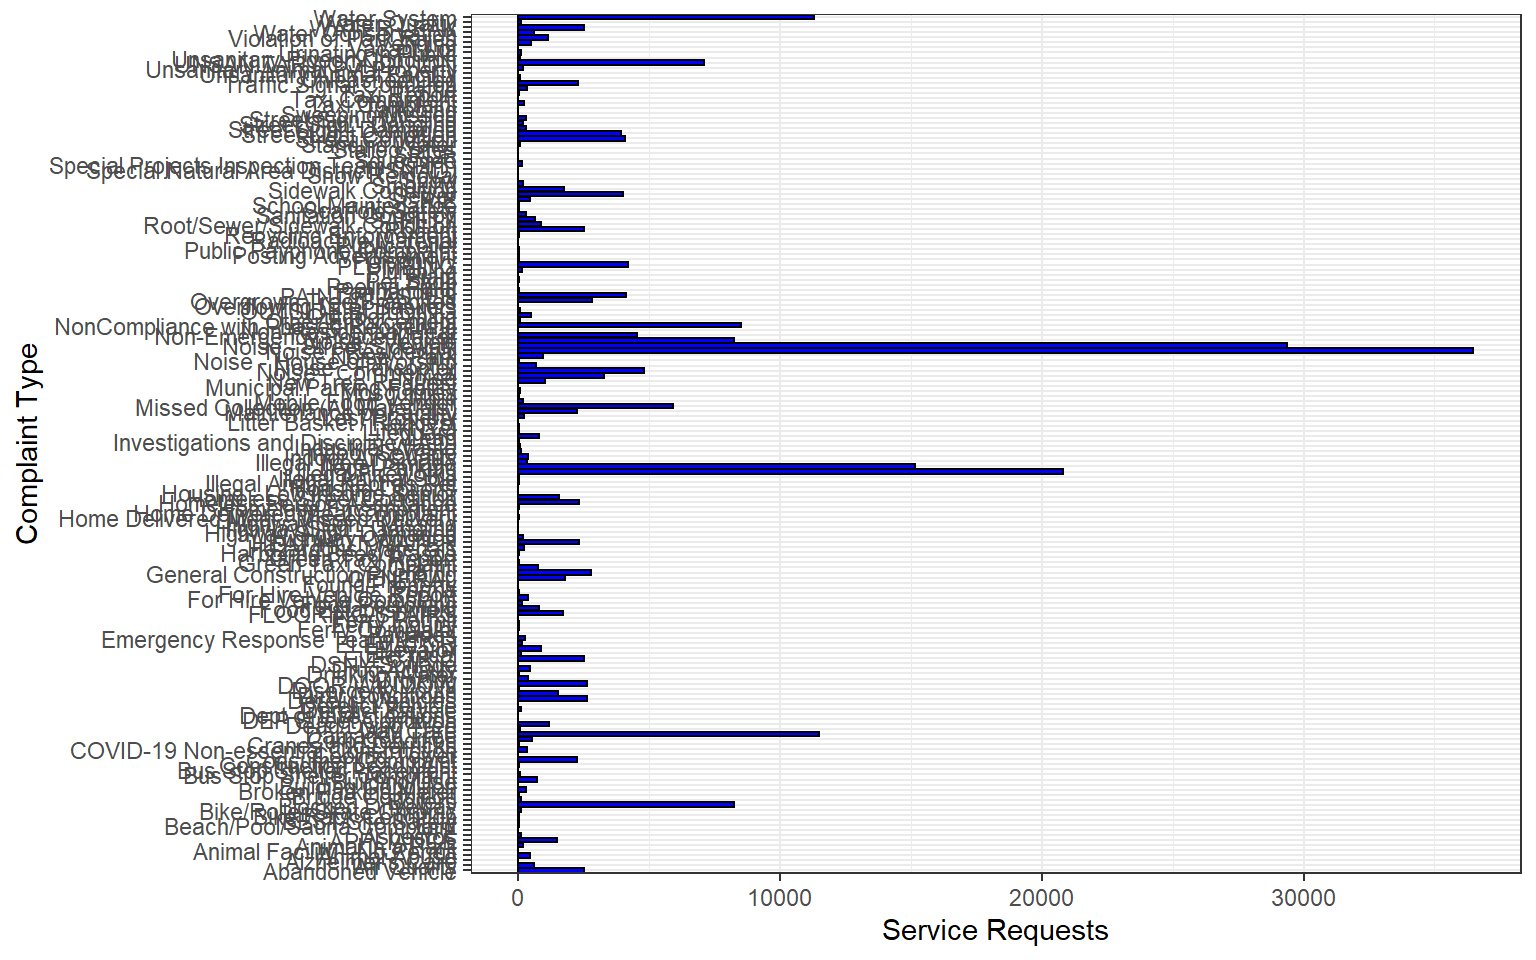
\includegraphics{traveler-multiple_regression_files/figure-latex/unnamed-chunk-4-1.pdf}

\begin{Shaded}
\begin{Highlighting}[]
\KeywordTok{summary}\NormalTok{(m_bty)}
\NormalTok{## }
\NormalTok{## Call:}
\NormalTok{## lm(formula = score ~ bty_avg, data = evals)}
\NormalTok{## }
\NormalTok{## Residuals:}
\NormalTok{##     Min      1Q  Median      3Q     Max }
\NormalTok{## -1.9246 -0.3690  0.1420  0.3977  0.9309 }
\NormalTok{## }
\NormalTok{## Coefficients:}
\NormalTok{##             Estimate Std. Error t value Pr(>|t|)    }
\NormalTok{## (Intercept)  3.88034    0.07614   50.96  < 2e-16 ***}
\NormalTok{## bty_avg      0.06664    0.01629    4.09 5.08e-05 ***}
\NormalTok{## ---}
\NormalTok{## Signif. codes:  0 '***' 0.001 '**' 0.01 '*' 0.05 '.' 0.1 ' ' 1}
\NormalTok{## }
\NormalTok{## Residual standard error: 0.5348 on 461 degrees of freedom}
\NormalTok{## Multiple R-squared:  0.03502,    Adjusted R-squared:  0.03293 }
\NormalTok{## F-statistic: 16.73 on 1 and 461 DF,  p-value: 5.083e-05}
\end{Highlighting}
\end{Shaded}

\section{JN: the equation is y = 0.06664 * x + 3.88034 // the slope
(0.06664) is positive, meaning every single increase in bty\_avg would
bring an increase of score by 0.06664. // Yes, the bty\_avg is a
significant predictor with p-value far below 0.05, i.e.~5.08e-05.
However, it may not be practically significant or useful because the
estimate is so small
(0.06664).}\label{jn-the-equation-is-y-0.06664-x-3.88034-the-slope-0.06664-is-positive-meaning-every-single-increase-in-bty_avg-would-bring-an-increase-of-score-by-0.06664.-yes-the-bty_avg-is-a-significant-predictor-with-p-value-far-below-0.05-i.e.5.08e-05.-however-it-may-not-be-practically-significant-or-useful-because-the-estimate-is-so-small-0.06664.}

\begin{enumerate}
\def\labelenumi{\arabic{enumi}.}
\setcounter{enumi}{5}
\tightlist
\item
  Use residual plots to evaluate whether the conditions of least squares
  regression are reasonable. Provide plots and comments for each one
  (see the Simple Regression Lab for a reminder of how to make these).
\end{enumerate}

\begin{Shaded}
\begin{Highlighting}[]
\KeywordTok{plot}\NormalTok{(m_bty}\OperatorTok{$}\NormalTok{residuals }\OperatorTok{~}\StringTok{ }\NormalTok{evals}\OperatorTok{$}\NormalTok{bty_avg)}
\KeywordTok{abline}\NormalTok{(}\DataTypeTok{h =} \DecValTok{0}\NormalTok{, }\DataTypeTok{lty =} \DecValTok{3}\NormalTok{)  }\CommentTok{# adds a horizontal dashed line at y = 0}
\end{Highlighting}
\end{Shaded}

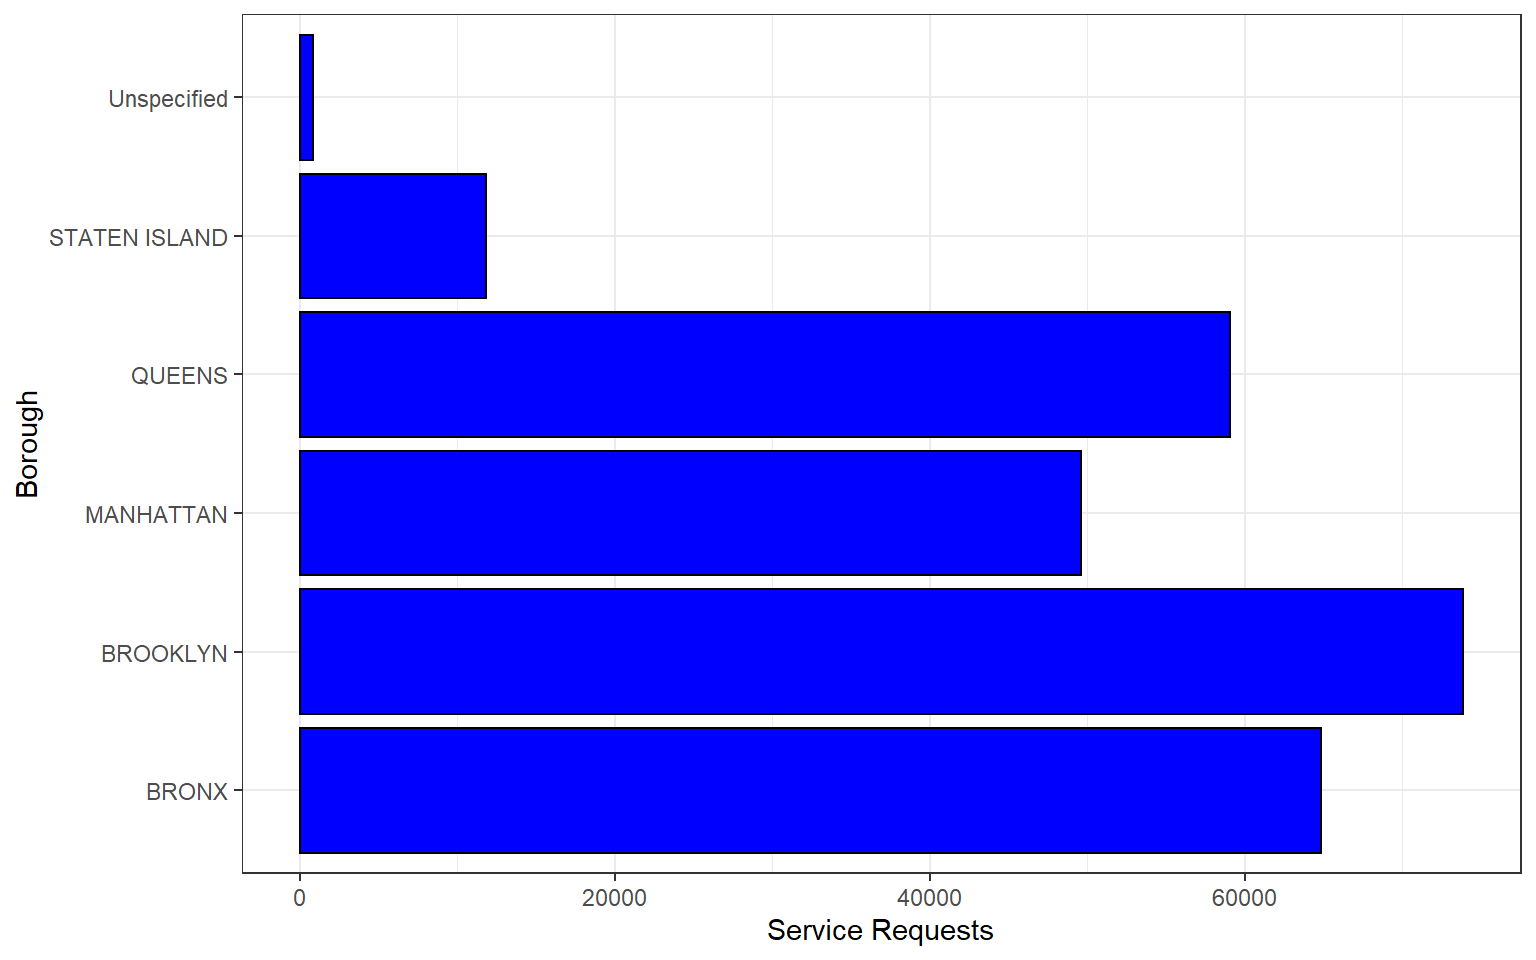
\includegraphics{traveler-multiple_regression_files/figure-latex/unnamed-chunk-5-1.pdf}
\# JN: yes the condition is met. The above residual plot shows a random
pattern - the randomness indicating the satisfaction of
homoscedasticity.

\subsection{Multiple linear
regression}\label{multiple-linear-regression}

The data set contains several variables on the beauty score of the
professor: individual ratings from each of the six students who were
asked to score the physical appearance of the professors and the average
of these six scores. Let's take a look at the relationship between one
of these scores and the average beauty score.

\begin{Shaded}
\begin{Highlighting}[]
\KeywordTok{plot}\NormalTok{(evals}\OperatorTok{$}\NormalTok{bty_avg }\OperatorTok{~}\StringTok{ }\NormalTok{evals}\OperatorTok{$}\NormalTok{bty_f1lower)}
\KeywordTok{cor}\NormalTok{(evals}\OperatorTok{$}\NormalTok{bty_avg, evals}\OperatorTok{$}\NormalTok{bty_f1lower)}
\end{Highlighting}
\end{Shaded}

As expected the relationship is quite strong - after all, the average
score is calculated using the individual scores. We can actually take a
look at the relationships between all beauty variables (columns 13
through 19) using the following command:

\begin{Shaded}
\begin{Highlighting}[]
\KeywordTok{plot}\NormalTok{(evals[,}\DecValTok{13}\OperatorTok{:}\DecValTok{19}\NormalTok{])}
\end{Highlighting}
\end{Shaded}

These variables are collinear (correlated), and adding more than one of
these variables to the model would not add much value to the model. In
this application and with these highly-correlated predictors, it is
reasonable to use the average beauty score as the single representative
of these variables.

In order to see if beauty is still a significant predictor of professor
score after we've accounted for the gender of the professor, we can add
the gender term into the model.

\begin{Shaded}
\begin{Highlighting}[]
\NormalTok{m_bty_gen <-}\StringTok{ }\KeywordTok{lm}\NormalTok{(score }\OperatorTok{~}\StringTok{ }\NormalTok{bty_avg }\OperatorTok{+}\StringTok{ }\NormalTok{gender, }\DataTypeTok{data =}\NormalTok{ evals)}
\KeywordTok{summary}\NormalTok{(m_bty_gen)}
\end{Highlighting}
\end{Shaded}

\begin{verbatim}
## 
## Call:
## lm(formula = score ~ bty_avg + gender, data = evals)
## 
## Residuals:
##     Min      1Q  Median      3Q     Max 
## -1.8305 -0.3625  0.1055  0.4213  0.9314 
## 
## Coefficients:
##             Estimate Std. Error t value Pr(>|t|)    
## (Intercept)  3.74734    0.08466  44.266  < 2e-16 ***
## bty_avg      0.07416    0.01625   4.563 6.48e-06 ***
## gendermale   0.17239    0.05022   3.433 0.000652 ***
## ---
## Signif. codes:  0 '***' 0.001 '**' 0.01 '*' 0.05 '.' 0.1 ' ' 1
## 
## Residual standard error: 0.5287 on 460 degrees of freedom
## Multiple R-squared:  0.05912,    Adjusted R-squared:  0.05503 
## F-statistic: 14.45 on 2 and 460 DF,  p-value: 8.177e-07
\end{verbatim}

\begin{enumerate}
\def\labelenumi{\arabic{enumi}.}
\setcounter{enumi}{6}
\tightlist
\item
  P-values and parameter estimates should only be trusted if the
  conditions for the regression are reasonable. Verify that the
  conditions for this model are reasonable using diagnostic plots.
\end{enumerate}

\begin{Shaded}
\begin{Highlighting}[]
\KeywordTok{library}\NormalTok{(car)}
\end{Highlighting}
\end{Shaded}

\begin{verbatim}
## Loading required package: carData
\end{verbatim}

\begin{Shaded}
\begin{Highlighting}[]
\KeywordTok{par}\NormalTok{(}\DataTypeTok{mfrow =} \KeywordTok{c}\NormalTok{(}\DecValTok{1}\NormalTok{, }\DecValTok{2}\NormalTok{))}
\KeywordTok{hist}\NormalTok{(m_bty_gen}\OperatorTok{$}\NormalTok{residuals, }\DataTypeTok{main =} \StringTok{"histogram of the residuals"}\NormalTok{)}
\NormalTok{car}\OperatorTok{::}\KeywordTok{qqPlot}\NormalTok{(m_bty_gen, }\DataTypeTok{main =} \StringTok{"qqplot of the residuals"}\NormalTok{)}
\end{Highlighting}
\end{Shaded}

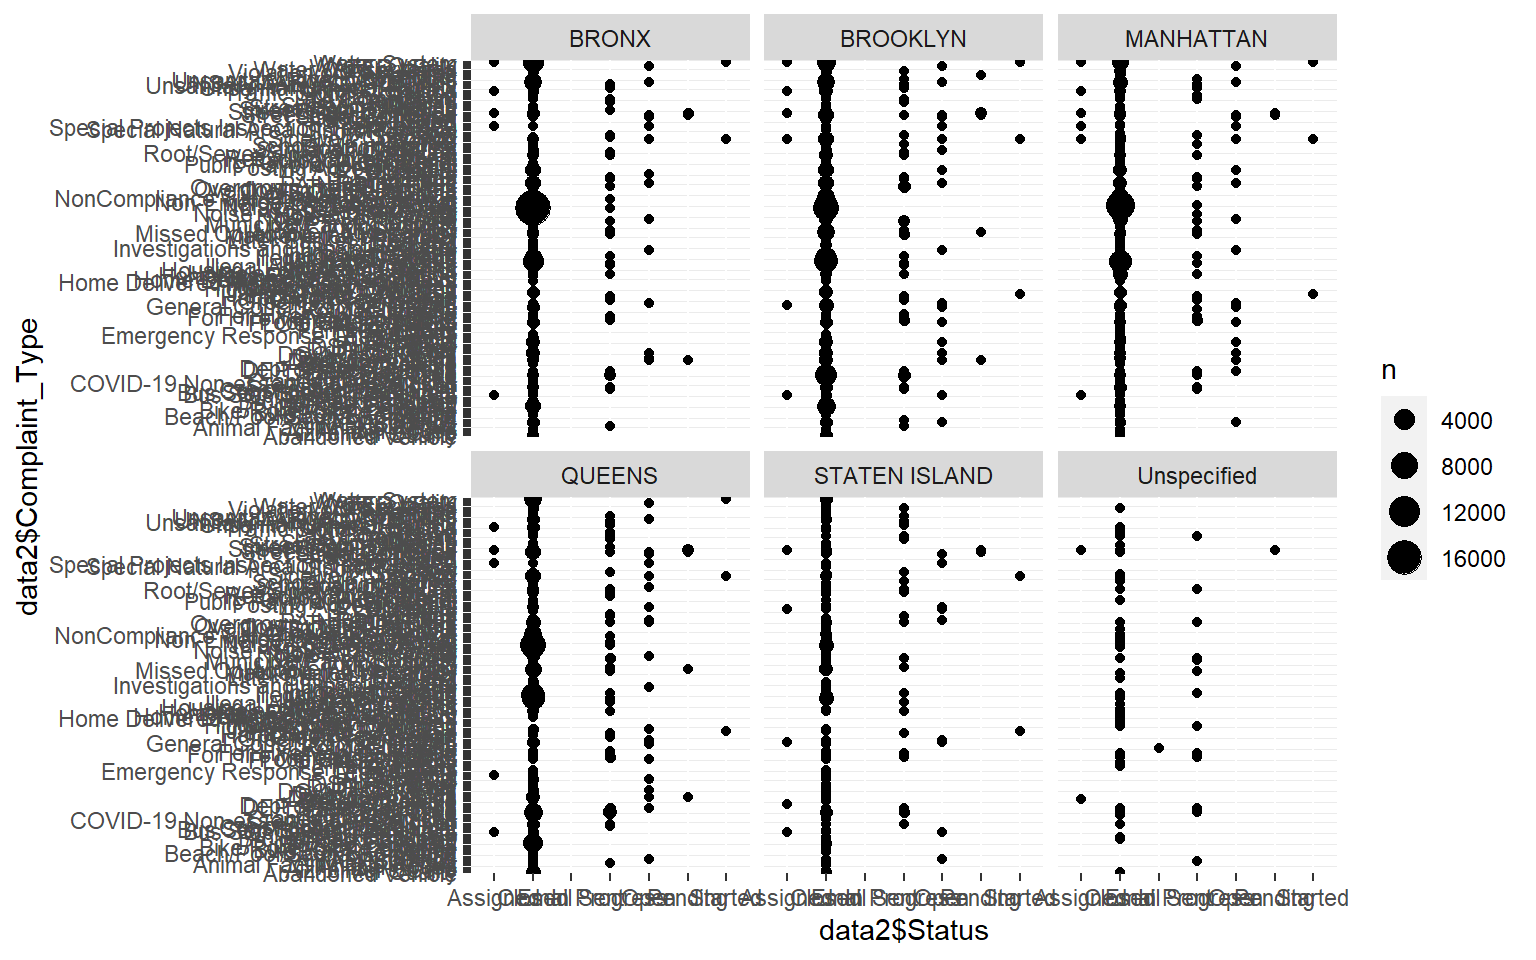
\includegraphics{traveler-multiple_regression_files/figure-latex/unnamed-chunk-6-1.pdf}

\begin{verbatim}
## [1] 162 335
\end{verbatim}

\section{JN: the residuals are nearly normally distributed (with left
skewed).}\label{jn-the-residuals-are-nearly-normally-distributed-with-left-skewed.}

\begin{enumerate}
\def\labelenumi{\arabic{enumi}.}
\setcounter{enumi}{7}
\tightlist
\item
  Is \texttt{bty\_avg} still a significant predictor of \texttt{score}?
  Has the addition of \texttt{gender} to the model changed the parameter
  estimate for \texttt{bty\_avg}? \# JN: Yes, it still is a significant
  predictor with p-value 6.48e-06. Adding ``gender'' to the model also
  changed the parameter estimate of ``bty\_avg'' from 0.06664 to
  0.07416.
\end{enumerate}

Note that the estimate for \texttt{gender} is now called
\texttt{gendermale}. You'll see this name change whenever you introduce
a categorical variable. The reason is that R recodes \texttt{gender}
from having the values of \texttt{female} and \texttt{male} to being an
indicator variable called \texttt{gendermale} that takes a value of
\(0\) for females and a value of \(1\) for males. (Such variables are
often referred to as ``dummy'' variables.)

As a result, for females, the parameter estimate is multiplied by zero,
leaving the intercept and slope form familiar from simple regression.

\[
  \begin{aligned}
\widehat{score} &= \hat{\beta}_0 + \hat{\beta}_1 \times bty\_avg + \hat{\beta}_2 \times (0) \\
&= \hat{\beta}_0 + \hat{\beta}_1 \times bty\_avg\end{aligned}
\]

We can plot this line and the line corresponding to males with the
following custom function.

\begin{Shaded}
\begin{Highlighting}[]
\KeywordTok{multiLines}\NormalTok{(m_bty_gen)}
\end{Highlighting}
\end{Shaded}

\begin{enumerate}
\def\labelenumi{\arabic{enumi}.}
\setcounter{enumi}{8}
\tightlist
\item
  What is the equation of the line corresponding to males? (\emph{Hint:}
  For males, the parameter estimate is multiplied by 1.) For two
  professors who received the same beauty rating, which gender tends to
  have the higher course evaluation score? \# JN: y = 3.74734 + x1 *
  (0.07416) + 1 * (0.17239). ``Male'' would tend to have higher score.
  If that's ``female'', the estimate (0.17239) would be multiplied by 0,
  and that means it will not be added or contributed to the increase in
  score.
\end{enumerate}

The decision to call the indicator variable \texttt{gendermale} instead
of\texttt{genderfemale} has no deeper meaning. R simply codes the
category that comes first alphabetically as a \(0\). (You can change the
reference level of a categorical variable, which is the level that is
coded as a 0, using the\texttt{relevel} function. Use \texttt{?relevel}
to learn more.)

\begin{enumerate}
\def\labelenumi{\arabic{enumi}.}
\setcounter{enumi}{9}
\tightlist
\item
  Create a new model called \texttt{m\_bty\_rank} with \texttt{gender}
  removed and \texttt{rank} added in. How does R appear to handle
  categorical variables that have more than two levels? Note that the
  rank variable has three levels: \texttt{teaching},
  \texttt{tenure\ track}, \texttt{tenured}.
\end{enumerate}

\begin{Shaded}
\begin{Highlighting}[]
\NormalTok{m_bty_rank <-}\StringTok{ }\KeywordTok{lm}\NormalTok{(score }\OperatorTok{~}\StringTok{ }\NormalTok{bty_avg }\OperatorTok{+}\StringTok{ }\NormalTok{rank, }\DataTypeTok{data =}\NormalTok{ evals)}
\KeywordTok{summary}\NormalTok{(m_bty_rank)}
\NormalTok{## }
\NormalTok{## Call:}
\NormalTok{## lm(formula = score ~ bty_avg + rank, data = evals)}
\NormalTok{## }
\NormalTok{## Residuals:}
\NormalTok{##     Min      1Q  Median      3Q     Max }
\NormalTok{## -1.8713 -0.3642  0.1489  0.4103  0.9525 }
\NormalTok{## }
\NormalTok{## Coefficients:}
\NormalTok{##                  Estimate Std. Error t value Pr(>|t|)    }
\NormalTok{## (Intercept)       3.98155    0.09078  43.860  < 2e-16 ***}
\NormalTok{## bty_avg           0.06783    0.01655   4.098 4.92e-05 ***}
\NormalTok{## ranktenure track -0.16070    0.07395  -2.173   0.0303 *  }
\NormalTok{## ranktenured      -0.12623    0.06266  -2.014   0.0445 *  }
\NormalTok{## ---}
\NormalTok{## Signif. codes:  0 '***' 0.001 '**' 0.01 '*' 0.05 '.' 0.1 ' ' 1}
\NormalTok{## }
\NormalTok{## Residual standard error: 0.5328 on 459 degrees of freedom}
\NormalTok{## Multiple R-squared:  0.04652,    Adjusted R-squared:  0.04029 }
\NormalTok{## F-statistic: 7.465 on 3 and 459 DF,  p-value: 6.88e-05}
\end{Highlighting}
\end{Shaded}

\section{\texorpdfstring{JN: the categorical variable would be
``dummified''. If it has 3 levels, then you will see it appear twice (k
- 1) as shown
above.}{JN: the categorical variable would be dummified. If it has 3 levels, then you will see it appear twice (k - 1) as shown above.}}\label{jn-the-categorical-variable-would-be-dummified.-if-it-has-3-levels-then-you-will-see-it-appear-twice-k---1-as-shown-above.}

The interpretation of the coefficients in multiple regression is
slightly different from that of simple regression. The estimate for
\texttt{bty\_avg} reflects how much higher a group of professors is
expected to score if they have a beauty rating that is one point higher
\emph{while holding all other variables constant}. In this case, that
translates into considering only professors of the same rank with
\texttt{bty\_avg} scores that are one point apart.

\subsection{The search for the best
model}\label{the-search-for-the-best-model}

We will start with a full model that predicts professor score based on
rank, ethnicity, gender, language of the university where they got their
degree, age, proportion of students that filled out evaluations, class
size, course level, number of professors, number of credits, average
beauty rating, outfit, and picture color.

\begin{enumerate}
\def\labelenumi{\arabic{enumi}.}
\setcounter{enumi}{10}
\tightlist
\item
  Which variable would you expect to have the highest p-value in this
  model? Why? \emph{Hint:} Think about which variable would you expect
  to not have any association with the professor score. \# JN: I expect
  that cls\_profs would have the highest p-value, simply because the
  number of professors teaching the course should have nothing to do
  with the score.
\end{enumerate}

Let's run the model\ldots{}

\begin{Shaded}
\begin{Highlighting}[]
\NormalTok{m_full <-}\StringTok{ }\KeywordTok{lm}\NormalTok{(score }\OperatorTok{~}\StringTok{ }\NormalTok{rank }\OperatorTok{+}\StringTok{ }\NormalTok{ethnicity }\OperatorTok{+}\StringTok{ }\NormalTok{gender }\OperatorTok{+}\StringTok{ }\NormalTok{language }\OperatorTok{+}\StringTok{ }\NormalTok{age }\OperatorTok{+}\StringTok{ }\NormalTok{cls_perc_eval }
             \OperatorTok{+}\StringTok{ }\NormalTok{cls_students }\OperatorTok{+}\StringTok{ }\NormalTok{cls_level }\OperatorTok{+}\StringTok{ }\NormalTok{cls_profs }\OperatorTok{+}\StringTok{ }\NormalTok{cls_credits }\OperatorTok{+}\StringTok{ }\NormalTok{bty_avg }
             \OperatorTok{+}\StringTok{ }\NormalTok{pic_outfit }\OperatorTok{+}\StringTok{ }\NormalTok{pic_color, }\DataTypeTok{data =}\NormalTok{ evals)}
\KeywordTok{summary}\NormalTok{(m_full)}
\end{Highlighting}
\end{Shaded}

\begin{enumerate}
\def\labelenumi{\arabic{enumi}.}
\setcounter{enumi}{11}
\item
  Check your suspicions from the previous exercise. Include the model
  output in your response. \# JN: Yes, my suspicion is confirmed -
  cls\_profssingle has the highest p-value of ``0.77806''. That means,
  the variable is highly irrelevant to the regression model.
\item
  Interpret the coefficient associated with the ethnicity variable. \#
  JN: once again, the p-value is not significant, i.e.~0.11698, meaning
  ethnicity of professor does not significantly impact the score. To
  interpret the coefficient, we can state that as when a professor is
  ``not minority'', we would add 0.1234929 to the score, holding
  everything else constant.
\item
  Drop the variable with the highest p-value and re-fit the model. Did
  the coefficients and significance of the other explanatory variables
  change? (One of the things that makes multiple regression interesting
  is that coefficient estimates depend on the other variables that are
  included in the model.) If not, what does this say about whether or
  not the dropped variable was collinear with the other explanatory
  variables?
\end{enumerate}

\begin{Shaded}
\begin{Highlighting}[]
\NormalTok{m_parital <-}\StringTok{ }\KeywordTok{lm}\NormalTok{(score }\OperatorTok{~}\StringTok{ }\NormalTok{rank }\OperatorTok{+}\StringTok{ }\NormalTok{ethnicity }\OperatorTok{+}\StringTok{ }\NormalTok{gender }\OperatorTok{+}\StringTok{ }\NormalTok{language }\OperatorTok{+}\StringTok{ }\NormalTok{age }\OperatorTok{+}\StringTok{ }\NormalTok{cls_perc_eval }
             \OperatorTok{+}\StringTok{ }\NormalTok{cls_students }\OperatorTok{+}\StringTok{ }\NormalTok{cls_level }\OperatorTok{+}\StringTok{ }\NormalTok{cls_credits }\OperatorTok{+}\StringTok{ }\NormalTok{bty_avg }
             \OperatorTok{+}\StringTok{ }\NormalTok{pic_outfit }\OperatorTok{+}\StringTok{ }\NormalTok{pic_color, }\DataTypeTok{data =}\NormalTok{ evals)}
\KeywordTok{summary}\NormalTok{(m_parital)}
\end{Highlighting}
\end{Shaded}

\section{\texorpdfstring{JN: Yes, the coefficients and significance of
the other explanatory variables change after dropping
``cls\_profs''.}{JN: Yes, the coefficients and significance of the other explanatory variables change after dropping cls\_profs.}}\label{jn-yes-the-coefficients-and-significance-of-the-other-explanatory-variables-change-after-dropping-cls_profs.}

\begin{enumerate}
\def\labelenumi{\arabic{enumi}.}
\setcounter{enumi}{14}
\tightlist
\item
  Using backward-selection and p-value as the selection criterion,
  determine the best model. You do not need to show all steps in your
  answer, just the output for the final model. Also, write out the
  linear model for predicting score based on the final model you settle
  on.
\end{enumerate}

\begin{Shaded}
\begin{Highlighting}[]
\NormalTok{m_all <-}\StringTok{ }\KeywordTok{lm}\NormalTok{(score }\OperatorTok{~}\NormalTok{., }\DataTypeTok{data =}\NormalTok{ evals)}

\KeywordTok{library}\NormalTok{(MASS)}
\NormalTok{MASS}\OperatorTok{::}\KeywordTok{stepAIC}\NormalTok{(m_all, }\DataTypeTok{direction =} \StringTok{"backward"}\NormalTok{)}
\NormalTok{## Start:  AIC=-631.44}
\NormalTok{## score ~ rank + ethnicity + gender + language + age + cls_perc_eval + }
\NormalTok{##     cls_did_eval + cls_students + cls_level + cls_profs + cls_credits + }
\NormalTok{##     bty_f1lower + bty_f1upper + bty_f2upper + bty_m1lower + bty_m1upper + }
\NormalTok{##     bty_m2upper + bty_avg + pic_outfit + pic_color}
\NormalTok{## }
\NormalTok{##                 Df Sum of Sq    RSS     AIC}
\NormalTok{## - cls_profs      1    0.0076 107.66 -633.41}
\NormalTok{## - cls_level      1    0.0756 107.73 -633.12}
\NormalTok{## - cls_students   1    0.1325 107.78 -632.87}
\NormalTok{## - bty_m2upper    1    0.1646 107.81 -632.73}
\NormalTok{## - bty_m1lower    1    0.1649 107.82 -632.73}
\NormalTok{## - bty_m1upper    1    0.1653 107.82 -632.73}
\NormalTok{## - bty_avg        1    0.1655 107.82 -632.73}
\NormalTok{## - bty_f1lower    1    0.1657 107.82 -632.73}
\NormalTok{## - bty_f2upper    1    0.1662 107.82 -632.73}
\NormalTok{## - bty_f1upper    1    0.1669 107.82 -632.72}
\NormalTok{## - cls_did_eval   1    0.1974 107.85 -632.59}
\NormalTok{## - pic_outfit     1    0.3270 107.98 -632.04}
\NormalTok{## <none>                       107.65 -631.44}
\NormalTok{## - rank           2    1.0319 108.68 -631.02}
\NormalTok{## - cls_perc_eval  1    0.5699 108.22 -631.00}
\NormalTok{## - ethnicity      1    0.9156 108.57 -629.52}
\NormalTok{## - language       1    1.2320 108.88 -628.17}
\NormalTok{## - age            1    1.5956 109.25 -626.63}
\NormalTok{## - pic_color      1    2.2190 109.87 -623.99}
\NormalTok{## - cls_credits    1    4.4803 112.13 -614.56}
\NormalTok{## - gender         1    5.6448 113.30 -609.78}
\NormalTok{## }
\NormalTok{## Step:  AIC=-633.41}
\NormalTok{## score ~ rank + ethnicity + gender + language + age + cls_perc_eval + }
\NormalTok{##     cls_did_eval + cls_students + cls_level + cls_credits + bty_f1lower + }
\NormalTok{##     bty_f1upper + bty_f2upper + bty_m1lower + bty_m1upper + bty_m2upper + }
\NormalTok{##     bty_avg + pic_outfit + pic_color}
\NormalTok{## }
\NormalTok{##                 Df Sum of Sq    RSS     AIC}
\NormalTok{## - cls_level      1    0.0751 107.73 -635.09}
\NormalTok{## - cls_students   1    0.1299 107.79 -634.85}
\NormalTok{## - bty_m2upper    1    0.1578 107.82 -634.73}
\NormalTok{## - bty_m1lower    1    0.1581 107.82 -634.73}
\NormalTok{## - bty_m1upper    1    0.1585 107.82 -634.73}
\NormalTok{## - bty_avg        1    0.1587 107.82 -634.73}
\NormalTok{## - bty_f1lower    1    0.1590 107.82 -634.72}
\NormalTok{## - bty_f2upper    1    0.1594 107.82 -634.72}
\NormalTok{## - bty_f1upper    1    0.1601 107.82 -634.72}
\NormalTok{## - cls_did_eval   1    0.1929 107.85 -634.58}
\NormalTok{## - pic_outfit     1    0.3673 108.03 -633.83}
\NormalTok{## <none>                       107.66 -633.41}
\NormalTok{## - rank           2    1.0311 108.69 -632.99}
\NormalTok{## - cls_perc_eval  1    0.5958 108.25 -632.85}
\NormalTok{## - ethnicity      1    0.9207 108.58 -631.47}
\NormalTok{## - language       1    1.2392 108.90 -630.11}
\NormalTok{## - age            1    1.6029 109.26 -628.57}
\NormalTok{## - pic_color      1    2.2156 109.87 -625.98}
\NormalTok{## - cls_credits    1    4.5061 112.16 -616.42}
\NormalTok{## - gender         1    5.6685 113.33 -611.65}
\NormalTok{## }
\NormalTok{## Step:  AIC=-635.09}
\NormalTok{## score ~ rank + ethnicity + gender + language + age + cls_perc_eval + }
\NormalTok{##     cls_did_eval + cls_students + cls_credits + bty_f1lower + }
\NormalTok{##     bty_f1upper + bty_f2upper + bty_m1lower + bty_m1upper + bty_m2upper + }
\NormalTok{##     bty_avg + pic_outfit + pic_color}
\NormalTok{## }
\NormalTok{##                 Df Sum of Sq    RSS     AIC}
\NormalTok{## - bty_m2upper    1    0.1353 107.87 -636.50}
\NormalTok{## - bty_m1lower    1    0.1356 107.87 -636.50}
\NormalTok{## - bty_m1upper    1    0.1359 107.87 -636.50}
\NormalTok{## - bty_avg        1    0.1361 107.87 -636.50}
\NormalTok{## - bty_f1lower    1    0.1364 107.87 -636.50}
\NormalTok{## - bty_f2upper    1    0.1368 107.87 -636.50}
\NormalTok{## - bty_f1upper    1    0.1374 107.87 -636.49}
\NormalTok{## - cls_students   1    0.1910 107.92 -636.27}
\NormalTok{## - cls_did_eval   1    0.2465 107.98 -636.03}
\NormalTok{## - pic_outfit     1    0.4078 108.14 -635.34}
\NormalTok{## <none>                       107.73 -635.09}
\NormalTok{## - rank           2    1.0007 108.73 -634.80}
\NormalTok{## - cls_perc_eval  1    0.5664 108.30 -634.66}
\NormalTok{## - ethnicity      1    0.9869 108.72 -632.86}
\NormalTok{## - language       1    1.1731 108.91 -632.07}
\NormalTok{## - age            1    1.5633 109.30 -630.41}
\NormalTok{## - pic_color      1    2.1435 109.88 -627.96}
\NormalTok{## - cls_credits    1    4.4849 112.22 -618.20}
\NormalTok{## - gender         1    5.6057 113.34 -613.60}
\NormalTok{## }
\NormalTok{## Step:  AIC=-636.5}
\NormalTok{## score ~ rank + ethnicity + gender + language + age + cls_perc_eval + }
\NormalTok{##     cls_did_eval + cls_students + cls_credits + bty_f1lower + }
\NormalTok{##     bty_f1upper + bty_f2upper + bty_m1lower + bty_m1upper + bty_avg + }
\NormalTok{##     pic_outfit + pic_color}
\NormalTok{## }
\NormalTok{##                 Df Sum of Sq    RSS     AIC}
\NormalTok{## - bty_m1lower    1    0.0319 107.90 -638.37}
\NormalTok{## - bty_m1upper    1    0.1637 108.03 -637.80}
\NormalTok{## - cls_students   1    0.2207 108.09 -637.56}
\NormalTok{## - cls_did_eval   1    0.2710 108.14 -637.34}
\NormalTok{## - pic_outfit     1    0.4084 108.28 -636.75}
\NormalTok{## <none>                       107.87 -636.50}
\NormalTok{## - bty_f1lower    1    0.4873 108.36 -636.42}
\NormalTok{## - cls_perc_eval  1    0.5417 108.41 -636.18}
\NormalTok{## - bty_avg        1    0.6009 108.47 -635.93}
\NormalTok{## - rank           2    1.1260 109.00 -635.70}
\NormalTok{## - ethnicity      1    0.8591 108.73 -634.83}
\NormalTok{## - language       1    1.1373 109.01 -633.65}
\NormalTok{## - bty_f2upper    1    1.1690 109.04 -633.51}
\NormalTok{## - age            1    1.5120 109.38 -632.06}
\NormalTok{## - bty_f1upper    1    1.8540 109.72 -630.61}
\NormalTok{## - pic_color      1    2.3311 110.20 -628.61}
\NormalTok{## - cls_credits    1    4.3939 112.26 -620.02}
\NormalTok{## - gender         1    5.8105 113.68 -614.21}
\NormalTok{## }
\NormalTok{## Step:  AIC=-638.37}
\NormalTok{## score ~ rank + ethnicity + gender + language + age + cls_perc_eval + }
\NormalTok{##     cls_did_eval + cls_students + cls_credits + bty_f1lower + }
\NormalTok{##     bty_f1upper + bty_f2upper + bty_m1upper + bty_avg + pic_outfit + }
\NormalTok{##     pic_color}
\NormalTok{## }
\NormalTok{##                 Df Sum of Sq    RSS     AIC}
\NormalTok{## - bty_m1upper    1    0.1347 108.03 -639.79}
\NormalTok{## - cls_students   1    0.2258 108.13 -639.40}
\NormalTok{## - cls_did_eval   1    0.2842 108.19 -639.15}
\NormalTok{## - pic_outfit     1    0.4271 108.33 -638.54}
\NormalTok{## <none>                       107.90 -638.37}
\NormalTok{## - bty_f1lower    1    0.5241 108.42 -638.12}
\NormalTok{## - cls_perc_eval  1    0.5243 108.42 -638.12}
\NormalTok{## - rank           2    1.0984 109.00 -637.68}
\NormalTok{## - ethnicity      1    0.9341 108.83 -636.38}
\NormalTok{## - language       1    1.1373 109.04 -635.51}
\NormalTok{## - bty_avg        1    1.1563 109.06 -635.43}
\NormalTok{## - bty_f2upper    1    1.4875 109.39 -634.03}
\NormalTok{## - age            1    1.6158 109.52 -633.49}
\NormalTok{## - bty_f1upper    1    2.3451 110.25 -630.41}
\NormalTok{## - pic_color      1    2.4870 110.39 -629.82}
\NormalTok{## - cls_credits    1    4.3675 112.27 -622.00}
\NormalTok{## - gender         1    5.8001 113.70 -616.13}
\NormalTok{## }
\NormalTok{## Step:  AIC=-639.79}
\NormalTok{## score ~ rank + ethnicity + gender + language + age + cls_perc_eval + }
\NormalTok{##     cls_did_eval + cls_students + cls_credits + bty_f1lower + }
\NormalTok{##     bty_f1upper + bty_f2upper + bty_avg + pic_outfit + pic_color}
\NormalTok{## }
\NormalTok{##                 Df Sum of Sq    RSS     AIC}
\NormalTok{## - cls_students   1    0.2111 108.25 -640.89}
\NormalTok{## - cls_did_eval   1    0.2718 108.31 -640.63}
\NormalTok{## - pic_outfit     1    0.4059 108.44 -640.05}
\NormalTok{## - bty_f1lower    1    0.4326 108.47 -639.94}
\NormalTok{## <none>                       108.03 -639.79}
\NormalTok{## - cls_perc_eval  1    0.6118 108.65 -639.18}
\NormalTok{## - rank           2    1.1107 109.15 -639.05}
\NormalTok{## - ethnicity      1    0.8677 108.90 -638.09}
\NormalTok{## - language       1    1.0897 109.12 -637.14}
\NormalTok{## - bty_avg        1    1.2696 109.31 -636.38}
\NormalTok{## - bty_f2upper    1    1.3535 109.39 -636.03}
\NormalTok{## - age            1    1.8207 109.86 -634.05}
\NormalTok{## - bty_f1upper    1    2.2334 110.27 -632.32}
\NormalTok{## - pic_color      1    2.5154 110.55 -631.13}
\NormalTok{## - cls_credits    1    4.8529 112.89 -621.45}
\NormalTok{## - gender         1    5.7018 113.74 -617.98}
\NormalTok{## }
\NormalTok{## Step:  AIC=-640.89}
\NormalTok{## score ~ rank + ethnicity + gender + language + age + cls_perc_eval + }
\NormalTok{##     cls_did_eval + cls_credits + bty_f1lower + bty_f1upper + }
\NormalTok{##     bty_f2upper + bty_avg + pic_outfit + pic_color}
\NormalTok{## }
\NormalTok{##                 Df Sum of Sq    RSS     AIC}
\NormalTok{## - cls_did_eval   1    0.1415 108.39 -642.28}
\NormalTok{## - pic_outfit     1    0.3573 108.60 -641.36}
\NormalTok{## - bty_f1lower    1    0.4667 108.71 -640.89}
\NormalTok{## <none>                       108.25 -640.89}
\NormalTok{## - rank           2    1.1821 109.43 -639.86}
\NormalTok{## - ethnicity      1    0.9919 109.24 -638.66}
\NormalTok{## - language       1    0.9963 109.24 -638.64}
\NormalTok{## - bty_avg        1    1.3404 109.59 -637.19}
\NormalTok{## - bty_f2upper    1    1.5770 109.82 -636.19}
\NormalTok{## - age            1    1.8395 110.09 -635.08}
\NormalTok{## - bty_f1upper    1    2.1827 110.43 -633.64}
\NormalTok{## - pic_color      1    2.3708 110.62 -632.85}
\NormalTok{## - cls_perc_eval  1    2.4497 110.70 -632.52}
\NormalTok{## - cls_credits    1    4.8839 113.13 -622.45}
\NormalTok{## - gender         1    5.5358 113.78 -619.79}
\NormalTok{## }
\NormalTok{## Step:  AIC=-642.28}
\NormalTok{## score ~ rank + ethnicity + gender + language + age + cls_perc_eval + }
\NormalTok{##     cls_credits + bty_f1lower + bty_f1upper + bty_f2upper + bty_avg + }
\NormalTok{##     pic_outfit + pic_color}
\NormalTok{## }
\NormalTok{##                 Df Sum of Sq    RSS     AIC}
\NormalTok{## <none>                       108.39 -642.28}
\NormalTok{## - pic_outfit     1    0.5065 108.89 -642.12}
\NormalTok{## - bty_f1lower    1    0.5212 108.91 -642.06}
\NormalTok{## - rank           2    1.2018 109.59 -641.18}
\NormalTok{## - ethnicity      1    1.0217 109.41 -639.94}
\NormalTok{## - language       1    1.0886 109.48 -639.65}
\NormalTok{## - bty_avg        1    1.4304 109.82 -638.21}
\NormalTok{## - bty_f2upper    1    1.7306 110.12 -636.95}
\NormalTok{## - age            1    1.9987 110.39 -635.82}
\NormalTok{## - pic_color      1    2.2613 110.65 -634.72}
\NormalTok{## - bty_f1upper    1    2.2891 110.68 -634.60}
\NormalTok{## - cls_perc_eval  1    2.3203 110.71 -634.47}
\NormalTok{## - cls_credits    1    4.9069 113.30 -623.78}
\NormalTok{## - gender         1    5.7484 114.14 -620.35}
\NormalTok{## }
\NormalTok{## Call:}
\NormalTok{## lm(formula = score ~ rank + ethnicity + gender + language + age + }
\NormalTok{##     cls_perc_eval + cls_credits + bty_f1lower + bty_f1upper + }
\NormalTok{##     bty_f2upper + bty_avg + pic_outfit + pic_color, data = evals)}
\NormalTok{## }
\NormalTok{## Coefficients:}
\NormalTok{##           (Intercept)       ranktenure track            ranktenured  }
\NormalTok{##               4.08717               -0.18412               -0.07980  }
\NormalTok{## ethnicitynot minority             gendermale    languagenon-english  }
\NormalTok{##               0.15616                0.25493               -0.22848  }
\NormalTok{##                   age          cls_perc_eval  cls_creditsone credit  }
\NormalTok{##              -0.00913                0.00447                0.50273  }
\NormalTok{##           bty_f1lower            bty_f1upper            bty_f2upper  }
\NormalTok{##               0.03884                0.07990                0.05849  }
\NormalTok{##               bty_avg   pic_outfitnot formal         pic_colorcolor  }
\NormalTok{##              -0.14036               -0.10030               -0.20547}
\end{Highlighting}
\end{Shaded}

\section{\texorpdfstring{JN: as shown above, we can use the \emph{AIC}
(Akaike's Information Criteria) to determine the best model. Using
direction = ``backward'' and starting with m\_all (by including every
explanatory variable), we found the best model (or stopped removing
variable) with the smallest AIC
returned.}{JN: as shown above, we can use the AIC (Akaike's Information Criteria) to determine the best model. Using direction = backward and starting with m\_all (by including every explanatory variable), we found the best model (or stopped removing variable) with the smallest AIC returned.}}\label{jn-as-shown-above-we-can-use-the-aic-akaikes-information-criteria-to-determine-the-best-model.-using-direction-backward-and-starting-with-m_all-by-including-every-explanatory-variable-we-found-the-best-model-or-stopped-removing-variable-with-the-smallest-aic-returned.}

And the model is described below,

lm(formula = score \textasciitilde{} rank + ethnicity + gender +
language + age + cls\_perc\_eval + cls\_credits + bty\_f1lower +
bty\_f1upper + bty\_f2upper + bty\_avg + pic\_outfit + pic\_color, data
= evals)

\begin{enumerate}
\def\labelenumi{\arabic{enumi}.}
\setcounter{enumi}{15}
\item
  Verify that the conditions for this model are reasonable using
  diagnostic plots.
\item
  The original paper describes how these data were gathered by taking a
  sample of professors from the University of Texas at Austin and
  including all courses that they have taught. Considering that each row
  represents a course, could this new information have an impact on any
  of the conditions of linear regression?
\item
  Based on your final model, describe the characteristics of a professor
  and course at University of Texas at Austin that would be associated
  with a high evaluation score.
\item
  Would you be comfortable generalizing your conclusions to apply to
  professors generally (at any university)? Why or why not?
\end{enumerate}

\hypertarget{license}{}
This is a product of OpenIntro that is released under a
\href{http://creativecommons.org/licenses/by-sa/3.0}{Creative Commons
Attribution-ShareAlike 3.0 Unported}. This lab was written by Mine
Çetinkaya-Rundel and Andrew Bray.


\end{document}
